\documentclass[12pt]{article}
\usepackage{note}

\title{Vector boson decay (tilt) angle probability}
\author{Ivan Pogrebnyak}
\date{\today}

\begin{document}
\maketitle

A vector boson, e.g. $W^-$, has spin $s^W=1$, with 3 possible projections on the quantization axis, $s^W_z=\pm 1,0$.
Consider a situation when a $W^-$ decays into 2 quarks, $\bar{u}$ and $d$. For concreteness, let the quantization axis $z$ be along the momentum vector of $W^-$ in the lab reference frame. With this choice of axes, the $W^-$ spin projection is its helicity.

The produced quarks both have spin $1/2$, and 2 possible spin projections on the $z'$ axis (along the momentum of $\bar{u}$), $s^q_{z'}=\pm 1/2$. But since the weak interactions all have left-handed chirality, the helicities of the product quarks are not random. The $d$ quark must be left-handed, $s^d_{z'}=1/2$, and the $\bar{u}$ quark must be right-handed, $s^u_{z'}=1/2$.

\begin{table}[H]\centering
\begin{tabular}{c|c c}
  Initial state & \multicolumn{2}{c}{Final state} \\ \hline
  $W$ & $\bar{u}$ & $d$ \\
  $s^W=1$ & $s^u=1/2$ & $s^d=1/2$ \\
  $s^W_z=\pm 1,0$ & $s^u_{z'}=1/2$ & $s^d_{z'}=1/2$ \\
\end{tabular}
\end{table}

By the triangle rule, the possible total final state spin values are
\begin{equation}
  \norm{s^u_{z'}-s^d_{z'}} \leq S^f \leq s^u_{z'}+s^d_{z'}
  \quad \Rightarrow \quad
  S^f = 0,1.
\end{equation}
%
But the total spin projection in the final state is
\begin{equation}
  S^f_{z'} = s^u_{z'} + s^d_{z'} = 1,
\end{equation}
which constrains the total spin to $S^f = 1$.

Thus, there are three possible initial states, each corresponding to a particular $W^-$ helicity, but only one final state. The amplitudes of overlap between the states are:
\begin{equation}\label{eq:overlap}
  \begin{array}{l}
    A_+ = \bracket{S^i=1,\, S^i_z= 1}{S^f=1,\, S^f_{z'}=1} = \bracket{\chi^i_+}{\chi'^f} \\
    A_0 = \bracket{S^i=1,\, S^i_z= 0}{S^f=1,\, S^f_{z'}=1} = \bracket{\chi^i_0}{\chi'^f} \\
    A_- = \bracket{S^i=1,\, S^i_z=-1}{S^f=1,\, S^f_{z'}=1} = \bracket{\chi^i_-}{\chi'^f}
  \end{array}
\end{equation}

To take the inner products, the initial and final state spinors need to be expressed in the same basis.
The transformation is given by the rotation operator,
\begin{equation}
  \hat{R}(\theta) : \chi'^f \mapsto \chi^f
\end{equation}
%
The rotation operator can be expressed in terms of the projection operator as
\begin{equation}\label{eq:RexpS}
  \hat{R}(\theta) = e^{-i\theta \hat{\vec{S}}\cdot\vec{n}}
  = e^{-i\theta \hat{S}_y}.
\end{equation}
Note, that we are interested in the passive rotation of the coordinates.

A definite projection state is an eigenstate of $\hat{S}_z$ with the projection as the eigenvalue. We can get the form of $\hat{S}_z$ directly from this statement, for an arbitrary spin:
\begin{equation}
  (\hat{S}_z)_{nm} = \bra{n}\hat{S}_z\ket{m} = m\bracket{n}{m} = m\delta_{nm}.
\end{equation}
%
Similarly%
\footnote{Problem 4.53 in J.D. Griffiths Quantum Mechanics (2nd ed.)}%
, to get $\hat{S}_x$ and $\hat{S}_y$, we use the raising and lowering operator eigenvalues
\begin{equation}
  (\hat{S}_\pm)_{nm} = \bra{n}\hat{S}_\pm\ket{m} = \sqrt{(s\mp m)(s\pm m+1)}\delta_{nm},
\end{equation}
and the definition of the raising and lowering operators,
\begin{equation}
  \hat{S}_x = \half(\hat{S}_+ + \hat{S}_-)
  \quad \text{and} \quad
  \hat{S}_y = \frac{1}{2i}(\hat{S}_+ - \hat{S}_-).
\end{equation}
%
Thus, the spin matrices for $S=1$ are
\begin{equation}
  \hat{S}_x = \frac{1}{\sqrt{2}}\begin{pmatrix}
    0 & 1 & 0 \\
    1 & 0 & 1 \\
    0 & 1 & 0
  \end{pmatrix}, \quad
  \hat{S}_y = \frac{1}{\sqrt{2}i}\begin{pmatrix}
    0 & 1 & 0 \\
   -1 & 0 & 1 \\
    0 &-1 & 0
  \end{pmatrix}, \quad
  \hat{S}_z = \begin{pmatrix}
    1 & 0 & 0 \\
    0 & 0 & 0 \\
    0 & 0 & -1
  \end{pmatrix}.
\end{equation}

Applying the Rodrigues' rotation formula
\begin{equation}
  e^{-i\theta\hat{S}_n} = \hat{1} - i\sin\theta\,\hat{S}_n - (1-\cos\theta)(\hat{S}_n)^2
\end{equation}
to \eq{RexpS}, we get
\begin{equation}
  \hat{R}(-\theta) = e^{-i\theta \hat{S}_y}
  = \begin{pmatrix}
    \half(1+\cos\theta) & -\frac{1}{\sqrt{2}}\sin\theta & \half(1-\cos\theta) \\
    \frac{1}{\sqrt{2}}\sin\theta & \cos\theta & -\frac{1}{\sqrt{2}}\sin\theta \\
    \half(1-\cos\theta) & \frac{1}{\sqrt{2}}\sin\theta & \half(1+\cos\theta) \\
  \end{pmatrix}.
\end{equation}

The overlap amplitudes defined in \eq{overlap} can now be found by
\begin{equation}\label{eq:overlap_found}
  \begin{array}{l}
    A_+ = \bracket{\chi^i_+}{\chi'^f}
%    = \bra{\chi^i_+}\hat{R}(\theta)\ket{\chi^f}
    = \bra{1}\hat{R}(\theta)\ket{1}
    = \half(1+\cos\theta) \\
    A_0 = \bracket{\chi^i_0}{\chi'^f}
    = \bra{0}\hat{R}(\theta)\ket{1}
    = \frac{1}{\sqrt{2}}\sin\theta \\
    A_- = \bracket{\chi^i_-}{\chi'^f}
    = \bra{-1}\hat{R}(\theta)\ket{1}
    = \half(1-\cos\theta)
  \end{array}
\end{equation}
%
We recognize these as the Wigner $d^J_{m,m'}$ functions for $J=1$,
\begin{equation}
  d^1_{1, 1} = \half[1+\cos\theta], \quad
  d^1_{1, 0} = \frac{\sin\theta}{\sqrt{2}}, \quad
  d^1_{1,-1} = \half[1-\cos\theta], \quad
  d^1_{0, 0} = \cos\theta.
\end{equation}

The probability of observing the corresponding decay product within a certain solid angle is given by
\begin{equation}\label{eq:angle_prob}
  P = c\int\! d\Omega\, \normsq{A(\theta)} = c\int\! d\phi\, \int\! d\theta\, \sin\theta \normsq{A(\theta)},
\end{equation}
which, by normalization condition, must integrate to unity over the whole solid angle of $4\pi$. The normalized probability density functions, $P_h(\theta)$, of decay at angle $\theta$ given a particular $W^-$ helicity are then:
\begin{equation}
  P_+(\theta) = \frac{3}{8}(1+\cos\theta)^2\sin\theta, \quad
  P_0(\theta) = \frac{3}{4}\sin^3\theta, \quad
  P_-(\theta) = \frac{3}{8}(1-\cos\theta)^2\sin\theta.
\end{equation}
%
These funstions are plotted below.

\vspace{-3mm}
\begin{figure}[H]
  \centering
  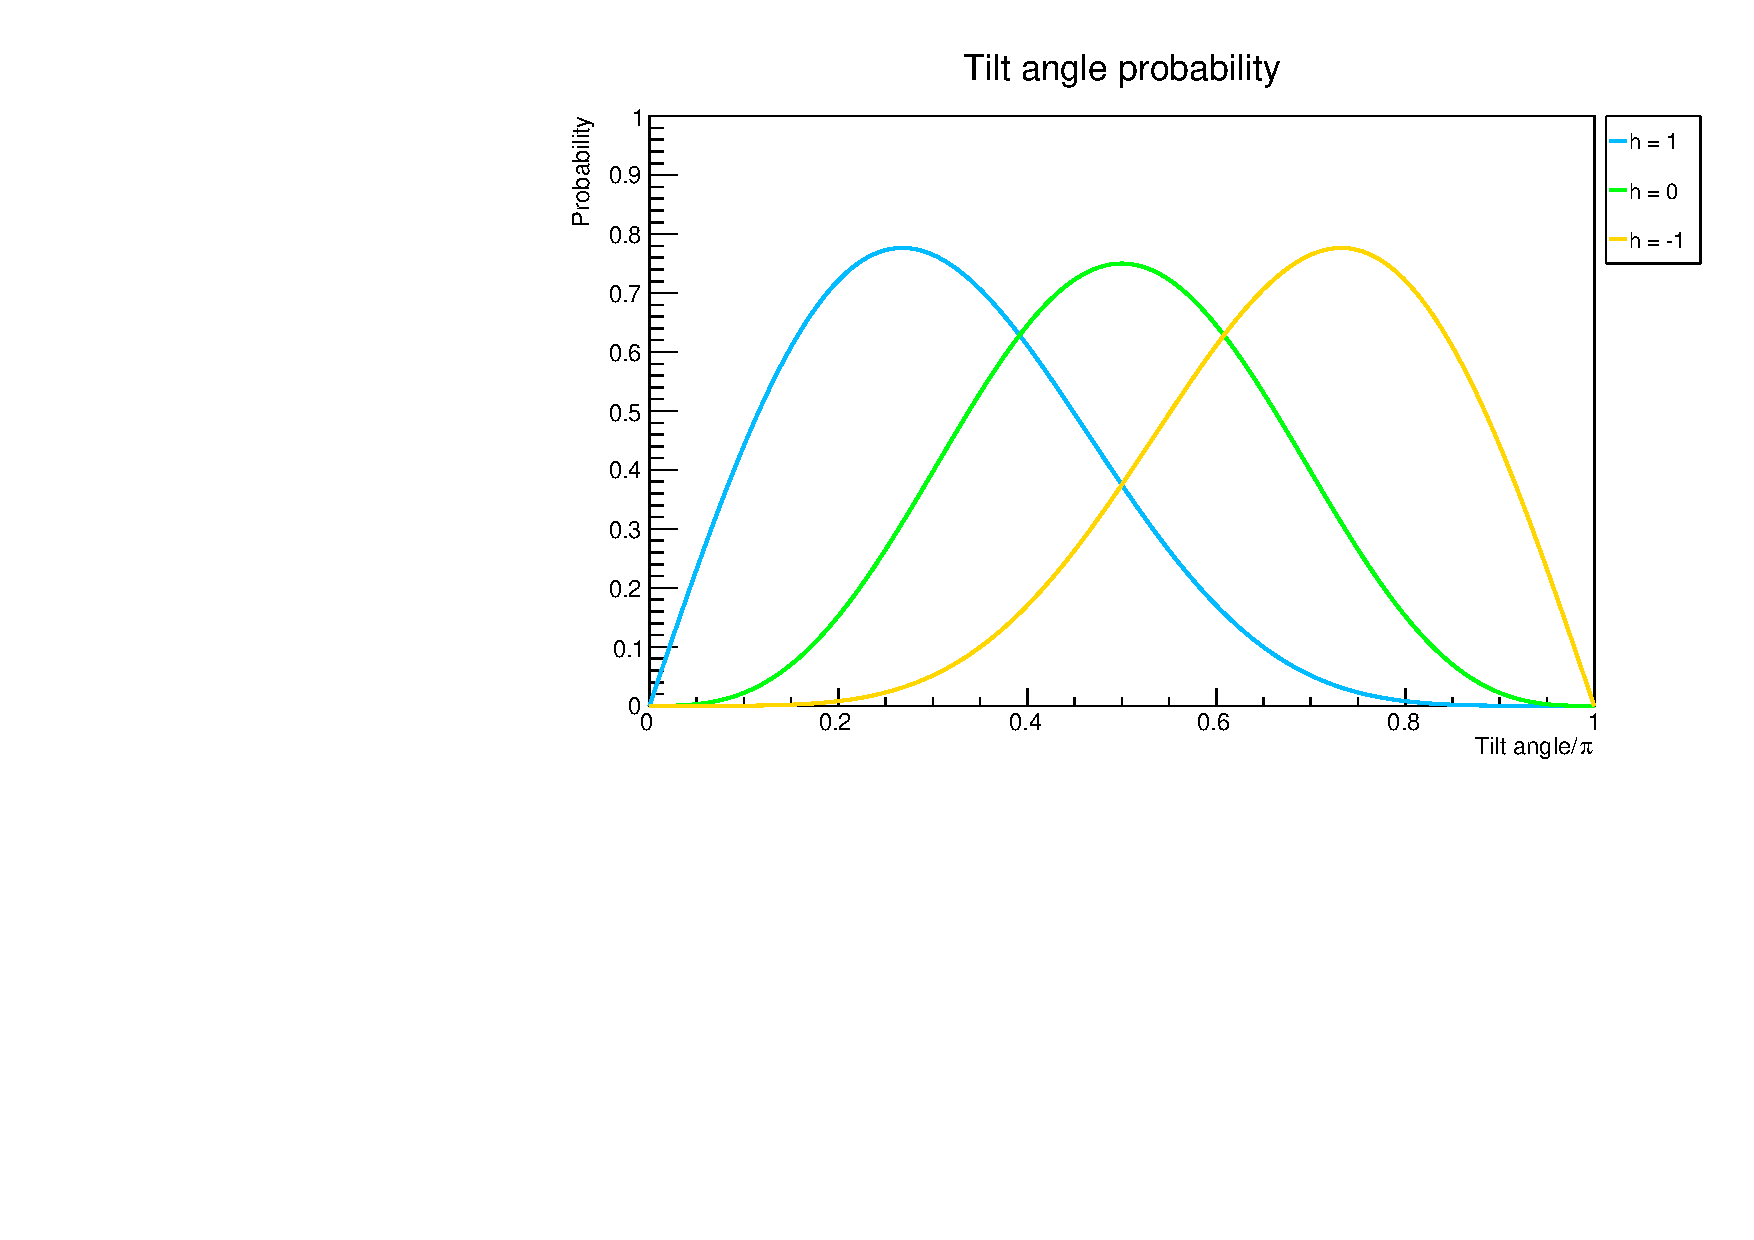
\includegraphics[width=0.95\textwidth]{fig/tilt_angle_prob.pdf}
\end{figure}

\vspace{-5mm}
Combining this result with the previously derived opening angle dependence on the tilt angle, we can find the opening angle probability density. This is plotted below for
$\gamma=2$. Note that the opening probability density functions are the same for helicity $\pm 1$, so only transversely and longitudinally polarized vector bosons can be distinguished. There plot has a cut off, because there is minimum opening angle allowed for a given $\gamma$.
\vspace{-3mm}
\begin{figure}[H]
  \centering
  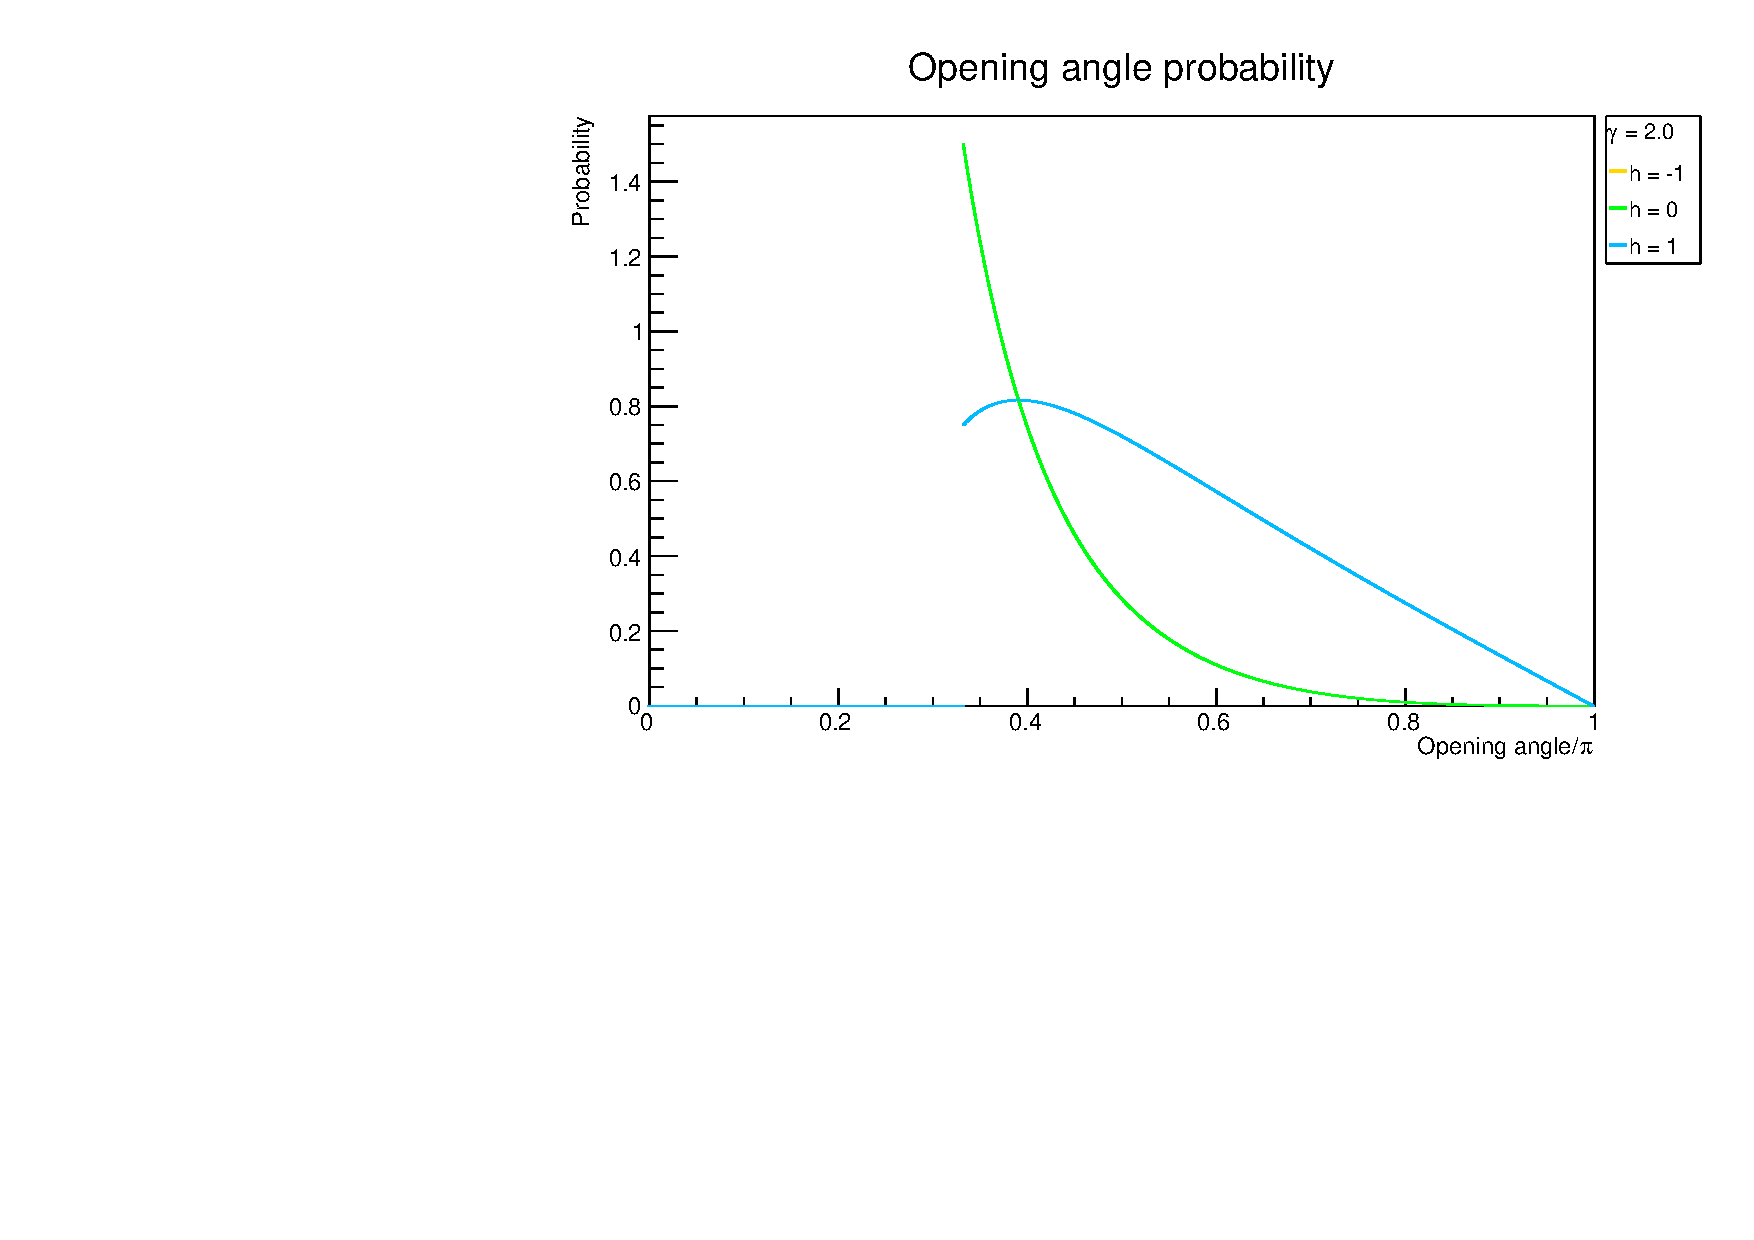
\includegraphics[width=0.95\textwidth]{fig/opening_angle_prob.pdf}
  \vspace{-10mm}
\end{figure}

To find the probability density of the cosine of the titl angle, we rewrite
\eq{angle_prob} as
\begin{equation}\label{eq:cos_prob}
  P = c\int_0^{2\pi}\! d\phi\, \int_{-1}^1\! d\cos\theta\, \normsq{A(\theta)}.
\end{equation}
The respective probability density functions are then,
\begin{equation}
  P_+(\cos\theta) = \frac{3}{8}(1+\cos\theta)^2, \quad
  P_0(\cos\theta) = \frac{3}{4}(1-\cos^2\theta), \quad
  P_-(\cos\theta) = \frac{3}{8}(1-\cos\theta)^2.
\end{equation}

\vspace{-3mm}
\begin{figure}[H]
  \centering
  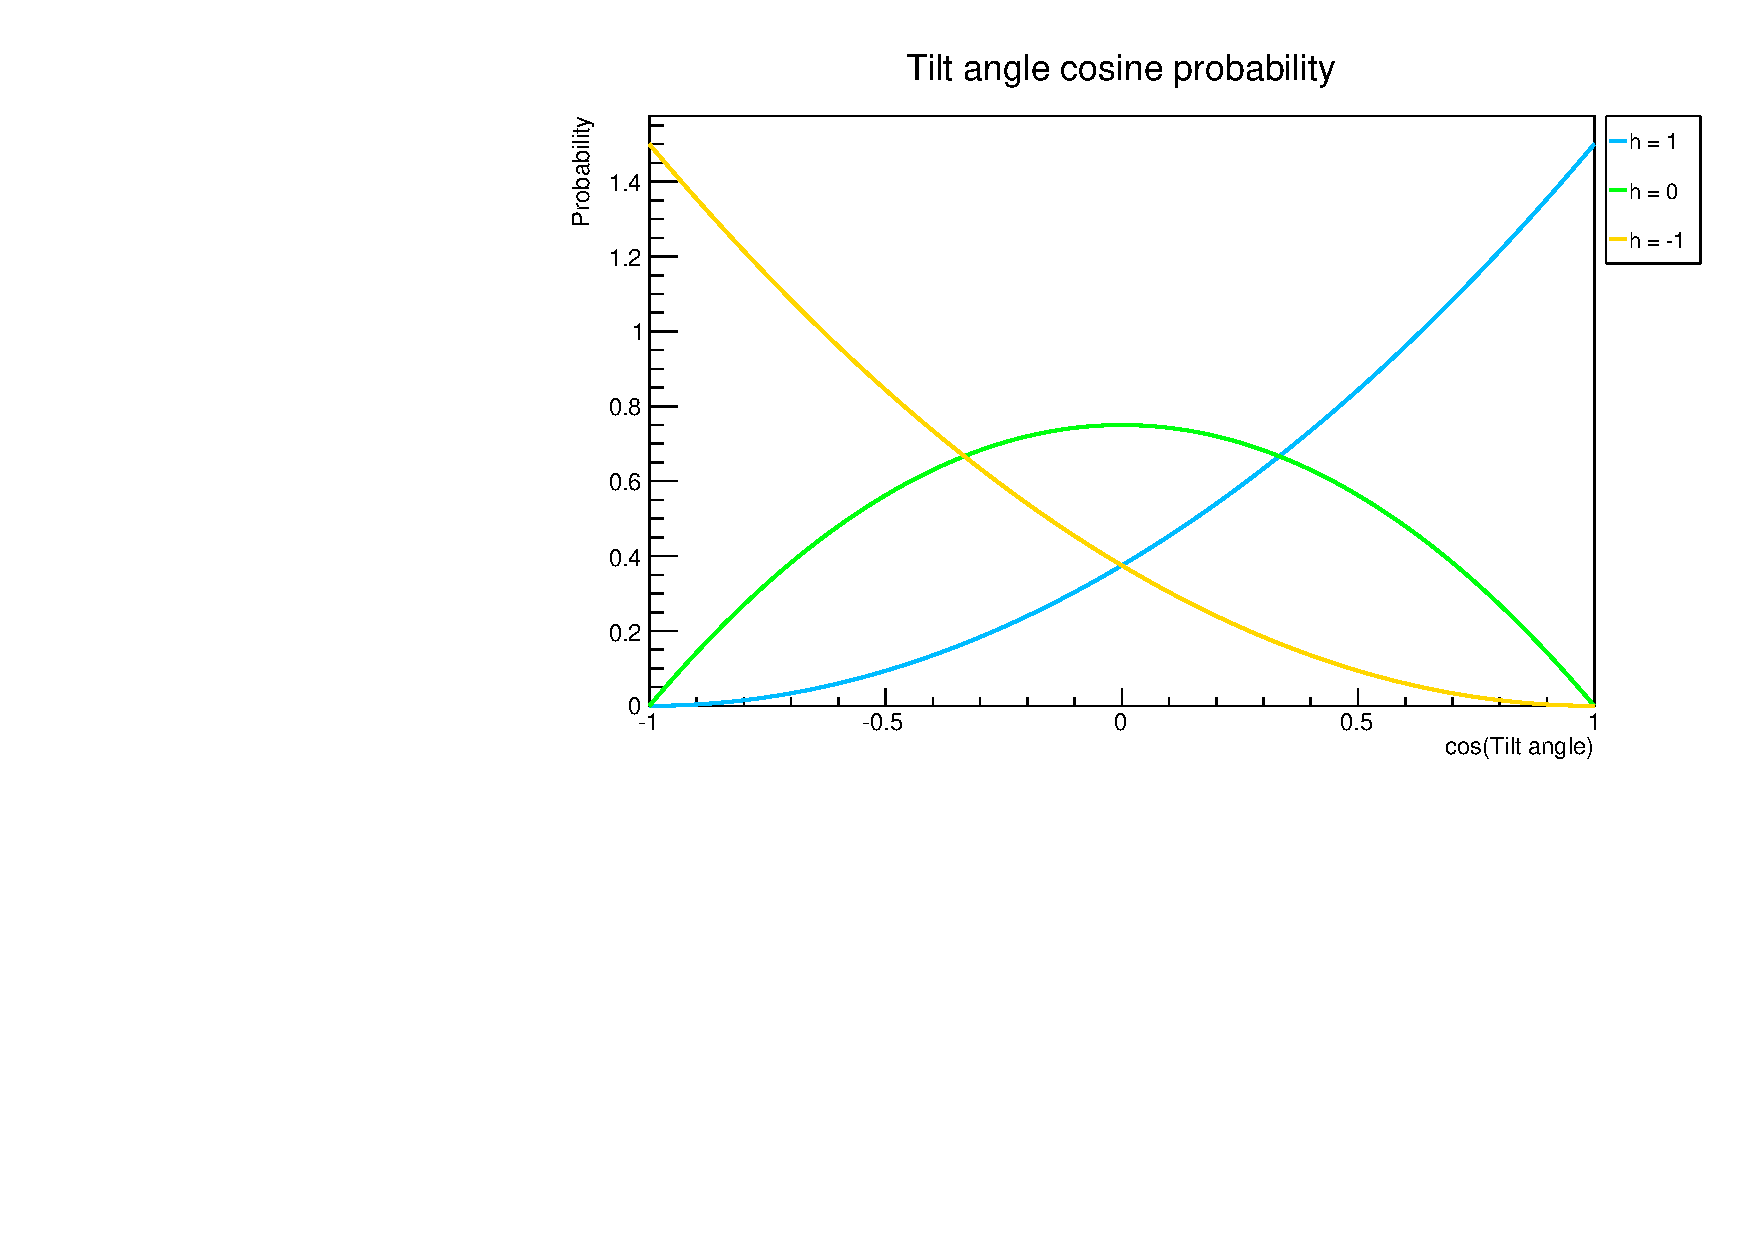
\includegraphics[width=0.95\textwidth]{fig/tilt_angle_cos_prob.pdf}
\end{figure}

\end{document}
